\documentclass[11pt,a4paper]{article}

% ── Packages ──────────────────────────────────────────────────────────────────
\usepackage[T1]{fontenc}
\usepackage[utf8]{inputenc}
\usepackage{lmodern}
\usepackage[margin=2.5cm]{geometry}
\usepackage{hyperref}
\usepackage{xcolor}
\usepackage{listings}
\usepackage{booktabs}
\usepackage{tabularx}
\usepackage{array}
\usepackage{enumitem}
\usepackage{amsmath}
\usepackage{graphicx}
\usepackage{microtype}
\usepackage{parskip}
\usepackage{titlesec}
\usepackage{abstract}
\usepackage{fancyhdr}
\usepackage{caption}
\usepackage{tikz}
\usetikzlibrary{shapes.geometric, arrows.meta, positioning, fit, backgrounds}

% ── Colours ───────────────────────────────────────────────────────────────────
\definecolor{agentbg}{HTML}{1a1a3a}
\definecolor{agentfg}{HTML}{c8c8ff}
\definecolor{agentborder}{HTML}{5858b0}
\definecolor{cpbg}{HTML}{2a1a0a}
\definecolor{cpfg}{HTML}{ffc060}
\definecolor{cpborder}{HTML}{c07820}
\definecolor{membg}{HTML}{1a0a2a}
\definecolor{memfg}{HTML}{c080ff}
\definecolor{memborder}{HTML}{8040c0}
\definecolor{codebg}{HTML}{0f0f1e}
\definecolor{codefg}{HTML}{c8d0e8}
\definecolor{codecomment}{HTML}{6272a4}
\definecolor{codestring}{HTML}{f1fa8c}
\definecolor{codekeyword}{HTML}{ff79c6}
\definecolor{linkcolor}{HTML}{8080d0}

% ── Hyperref ──────────────────────────────────────────────────────────────────
\hypersetup{
  colorlinks=true,
  linkcolor=linkcolor,
  urlcolor=linkcolor,
  citecolor=linkcolor,
  pdftitle={ApolloAgents: A Multi-Agent Architecture for Autonomous DJ Set Generation},
  pdfauthor={Pablo Formoso},
}

% ── Code listings ─────────────────────────────────────────────────────────────
\lstdefinestyle{apollo}{
  backgroundcolor=\color{codebg},
  basicstyle=\ttfamily\small\color{codefg},
  commentstyle=\color{codecomment}\itshape,
  keywordstyle=\color{codekeyword}\bfseries,
  stringstyle=\color{codestring},
  breaklines=true,
  breakatwhitespace=true,
  frame=single,
  framesep=6pt,
  rulecolor=\color{agentborder},
  xleftmargin=10pt,
  xrightmargin=10pt,
  tabsize=4,
  showstringspaces=false,
  numbers=none,
}
\lstset{style=apollo}

% ── Section formatting ────────────────────────────────────────────────────────
\titleformat{\section}{\large\bfseries}{\thesection.}{0.6em}{}[\vspace{-0.3em}\rule{\linewidth}{0.4pt}]
\titleformat{\subsection}{\normalsize\bfseries}{\thesubsection}{0.6em}{}
\titleformat{\subsubsection}{\normalsize\itshape}{\thesubsubsection}{0.6em}{}

% ── Header / footer ───────────────────────────────────────────────────────────
\pagestyle{fancy}
\fancyhf{}
\rhead{\small ApolloAgents — Multi-Agent DJ Architecture}
\lhead{\small Formoso, 2026}
\rfoot{\small \thepage}
\renewcommand{\headrulewidth}{0.3pt}

% ── TikZ styles ───────────────────────────────────────────────────────────────
\tikzstyle{agent} = [rectangle, rounded corners=4pt,
  fill=agentbg, draw=agentborder, text=agentfg,
  font=\ttfamily\footnotesize, align=center,
  inner sep=6pt, minimum width=3.8cm, minimum height=1.1cm]

\tikzstyle{checkpoint} = [diamond, aspect=2.5,
  fill=cpbg, draw=cpborder, text=cpfg,
  font=\ttfamily\footnotesize, align=center,
  inner sep=3pt]

\tikzstyle{memory} = [ellipse,
  fill=membg, draw=memborder, text=memfg,
  font=\ttfamily\footnotesize, align=center,
  inner sep=5pt]

\tikzstyle{arrow} = [-{Stealth[length=5pt]}, color=agentborder, thick]
\tikzstyle{dasharrow} = [-{Stealth[length=5pt]}, color=memborder, dashed, thick]

% ── Document ──────────────────────────────────────────────────────────────────
\begin{document}

% ── Title ─────────────────────────────────────────────────────────────────────
\begin{center}
  {\LARGE\bfseries ApolloAgents: A Multi-Agent Architecture\\[4pt]
  for Autonomous DJ Set Generation}\\[14pt]
  {\large Pablo Formoso}\\[4pt]
  {\normalsize Independent Research \quad\textbullet\quad April 2026}\\[4pt]
  {\small\url{https://github.com/pabloformoso/apollo-agents}}
\end{center}

\vspace{6pt}\rule{\linewidth}{0.6pt}\vspace{6pt}

% ── Abstract ──────────────────────────────────────────────────────────────────
\begin{abstract}
This paper presents ApolloAgents, an AI-powered system that transforms a
collection of audio tracks into a fully rendered DJ mix video through a
coordinated pipeline of specialised language model agents. The system
addresses the inherent complexity of DJ set curation --- harmonic
compatibility, energy arc design, rhythmic continuity, and audio quality ---
by decomposing the problem across agents with distinct, bounded roles: a
Genre Guard, a Catalog Manager, a Planner, a Critic, a Validator, and a
human-in-the-loop Orchestrator. Each agent communicates through structured
text protocols and a shared context object, avoiding the overhead of
distributed message buses while preserving the modularity benefits of
multi-agent design. A persistent session memory allows agents to learn from
past sessions, progressively improving track avoidance, energy arc selection,
and transition quality over time. Version 1.3 extends the pipeline with BPM
stretch safety bounds, bridge track insertion tooling, and crossfade EQ
matching to reduce frequency masking at transitions. Version 1.5 introduces
LiveMode --- a real-time DJ engine backed by a proactive LiveDJ agent that
monitors the active mix and makes autonomous transition decisions, extending
the system from a batch pipeline to a real-time interactive performance tool.
The full pipeline --- from prompt to lossless WAV mix to 1080p YouTube video
with AI-generated artwork --- runs without human intervention beyond two
interactive checkpoints.
\end{abstract}

\vspace{6pt}\rule{\linewidth}{0.6pt}\vspace{10pt}

% ─────────────────────────────────────────────────────────────────────────────
\section{Introduction}
% ─────────────────────────────────────────────────────────────────────────────

Creating a DJ mix is a compositional act that balances multiple musical
dimensions simultaneously. A skilled DJ considers harmonic compatibility
between tracks (so key changes do not clash), BPM continuity (so tempo
transitions feel natural rather than jarring), energy arc (so the set has a
narrative shape --- warmup, build, peak, release), and audio quality (so no
individual track bleaches, clips, or drops into silence). This is a rich,
multi-constraint optimisation problem that resists reduction to a single
prompt or a simple ranking function.

Large language models excel at tasks requiring structured reasoning,
preference modelling, and natural language interaction. However, a single
general-purpose agent asked to ``plan a 60-minute techno set'' will tend to
produce superficially plausible but musically shallow results: it lacks the
domain specificity to analyse harmonic wheels, the numerical grounding to
evaluate BPM clusters, and the self-critical distance to review its own
choices objectively.

ApolloAgents decomposes the problem into a pipeline of agents, each
specialised for a single phase of the workflow. This mirrors professional DJ
practice: a promoter confirms the brief, a music researcher curates the
catalog, a set planner proposes a running order, an A\&R person critiques it,
and an engineer handles the technical render. The system encodes this division
of labour into distinct agents with clearly bounded system prompts, tool
access, and output formats.

\medskip
The contributions of this work are:

\begin{enumerate}[leftmargin=*, label=\arabic*.]
  \item A practical multi-agent architecture for creative audio production,
        implemented without orchestration frameworks
  \item A structured text protocol for inter-agent communication (CONFIRMED
        blocks, PROBLEMS/VERDICT format, Status: fields)
  \item A lossless audio pipeline addressing the crossfade clipping problem
        endemic to na\"ive pydub-based mixing
  \item A persistent session memory that allows agents to improve
        recommendations based on accumulated user feedback
  \item A full video production pipeline integrating spectral waveform
        visualisation, beat-reactive particles, and AI-generated artwork
  \item BPM stretch safety bounds and bridge track insertion tooling (v1.3)
        that prevent time-stretching artefacts and give the Editor agent a
        structured path to resolve extreme tempo gaps
  \item A real-time proactive DJ agent (LiveDJ, v1.5) that monitors a live
        mix in progress and makes autonomous transition decisions within a
        bounded LLM turn budget
\end{enumerate}

% ─────────────────────────────────────────────────────────────────────────────
\section{Background}
% ─────────────────────────────────────────────────────────────────────────────

\subsection{The Camelot Wheel}

The Camelot Wheel is a harmonic mixing reference system developed by Mark
Davis~\cite{davis2004} that maps Western musical keys onto a clock face. Each
position represents a key (e.g., 8A = A minor, 8B = C major). Two tracks are
considered harmonically compatible if their Camelot positions are:

\begin{itemize}
  \item \textbf{Identical} --- same key, always safe
  \item \textbf{Adjacent by number} ($\pm$1) --- relative key shift, smooth transition
  \item \textbf{Adjacent by letter} (A$\leftrightarrow$B at same number) ---
        parallel major/minor, slightly bolder
\end{itemize}

Transitions two steps apart are acceptable with technique; larger jumps risk
audible key clash. ApolloAgents encodes this as a graph neighbour function:

\begin{lstlisting}[language=Python]
def _camelot_neighbors(key: str) -> set[str]:
    num = int(key[:-1])
    letter = key[-1].upper()
    opposite = "B" if letter == "A" else "A"
    return {
        key,
        f"{(num % 12) + 1}{letter}",        # +1 clockwise
        f"{((num - 2) % 12) + 1}{letter}",  # -1 counter-clockwise
        f"{num}{opposite}",                  # parallel key
    }
\end{lstlisting}

The harmonic sort algorithm performs a greedy random walk on this graph to
produce a compatible running order from a pool of clustered tracks.

\subsection{BPM Matching}

Professional DJ mixing involves beatmatching: aligning the tempo of the
incoming track to the outgoing track before the crossfade begins.
ApolloAgents implements tempo matching via \texttt{pyrubberband}~\cite{rubberband},
a Python wrapper around the Rubber Band Library which uses phase-vocoder
time-stretching to change playback speed without altering pitch. Tracks within
\texttt{BPM\_MATCH\_THRESHOLD} (5 BPM) are played at their native tempo;
larger differences trigger a 16-second ramp (\texttt{TEMPO\_RAMP\_SEC}) that
linearly interpolates BPM across \texttt{RAMP\_STEPS = 24} micro-segments for
a smooth transition.

\subsection{The Crossfade Clipping Problem}

A widely overlooked issue in programmatic mixing is that crossfading two audio
signals at full amplitude causes additive clipping. If both tracks peak at
0~dBFS, their sum during overlap reaches +6~dBFS --- beyond the representable
range --- producing digital distortion. The system addresses this with two
mitigations:

\begin{enumerate}
  \item \textbf{Pre-mix gain reduction}: every track is attenuated by $-3$~dB
        before mixing (\texttt{segment = segment - 3})
  \item \textbf{Post-mix normalisation}: if the final mix peaks below
        $-1$~dBFS, it is normalised to recover headroom
\end{enumerate}

Additionally, per-crossfade peak monitoring warns when the overlap zone
exceeds $-0.5$~dBFS, allowing detection without requiring a full librosa
analysis pass.

\subsection{Multi-Agent Systems for Creative Tasks}

Prior work has explored LLM agents for creative generation in domains
including code synthesis, game design, and narrative writing. The
ApolloAgents architecture draws inspiration from the AutoAgent pattern of
specialised subagents with bounded tool access~\cite{autoagent}, but
implements it directly against the Anthropic and OpenAI APIs rather than
relying on an orchestration framework. This keeps the dependency surface
minimal and makes the control flow inspectable in a single file.

% ─────────────────────────────────────────────────────────────────────────────
\section{System Architecture}
% ─────────────────────────────────────────────────────────────────────────────

\subsection{Overview}

ApolloAgents structures the mix creation process as an 8-phase sequential
pipeline. Each phase is handled by a dedicated agent with a fixed system
prompt, a curated subset of tools, and a structured output format. Shared
mutable state is carried in a \texttt{context\_variables} dictionary injected
by the orchestrator.

\begin{figure}[h]
\centering
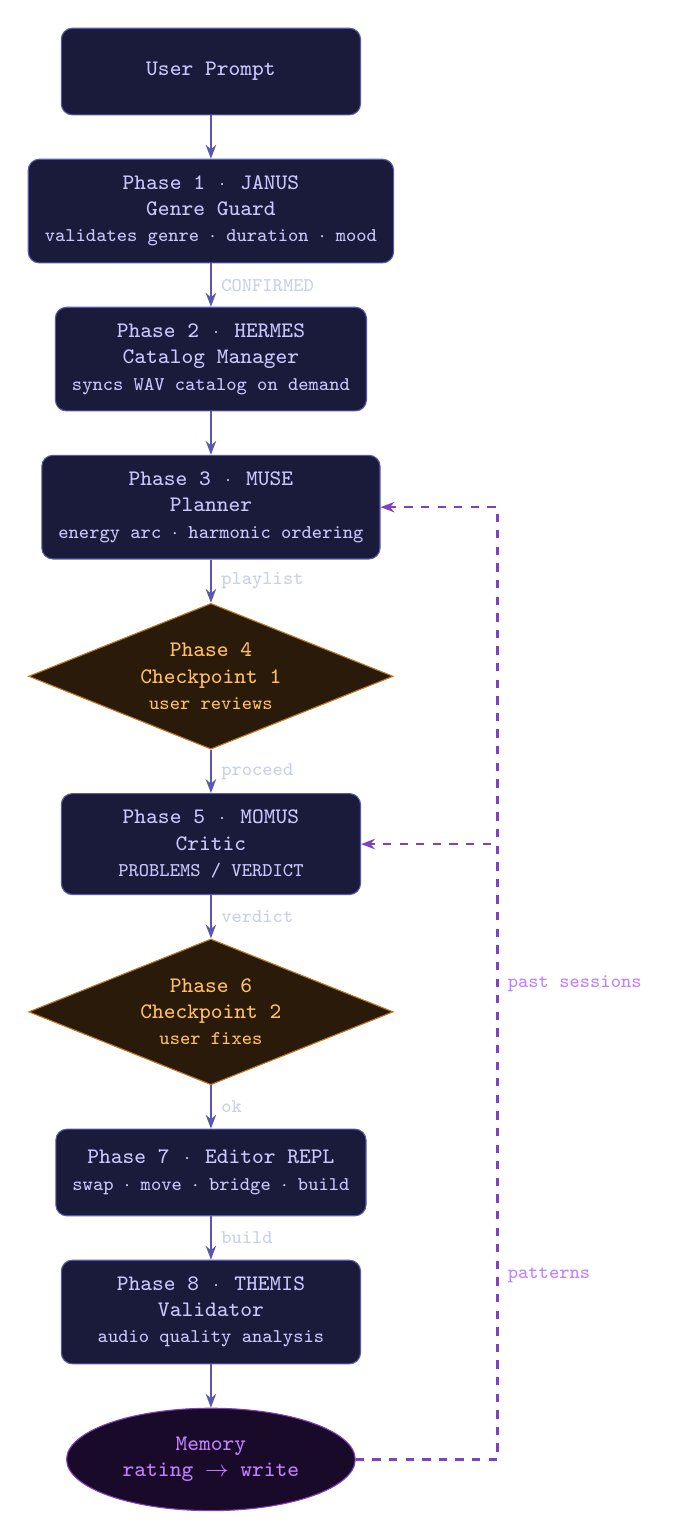
\begin{tikzpicture}[node distance=0.55cm and 2.2cm]

  \node[agent] (user) {\textbf{User Prompt}};

  \node[agent, below=of user] (p1)
    {\textbf{Phase 1 · JANUS}\\Genre Guard\\{\scriptsize validates genre $\cdot$ duration $\cdot$ mood}};

  \node[agent, below=of p1] (p2)
    {\textbf{Phase 2 · HERMES}\\Catalog Manager\\{\scriptsize syncs WAV catalog on demand}};

  \node[agent, below=of p2] (p3)
    {\textbf{Phase 3 · MUSE}\\Planner\\{\scriptsize energy arc $\cdot$ harmonic ordering}};

  \node[checkpoint, below=of p3] (cp1)
    {\textbf{Phase 4}\\Checkpoint 1\\{\scriptsize user reviews}};

  \node[agent, below=of cp1] (p5)
    {\textbf{Phase 5 · MOMUS}\\Critic\\{\scriptsize PROBLEMS / VERDICT}};

  \node[checkpoint, below=of p5] (cp2)
    {\textbf{Phase 6}\\Checkpoint 2\\{\scriptsize user fixes}};

  \node[agent, below=of cp2] (p7)
    {\textbf{Phase 7 · Editor REPL}\\{\scriptsize swap $\cdot$ move $\cdot$ bridge $\cdot$ build}};

  \node[agent, below=of p7] (p8)
    {\textbf{Phase 8 · THEMIS}\\Validator\\{\scriptsize audio quality analysis}};

  \node[memory, below=of p8] (mem)
    {\textbf{Memory}\\rating $\rightarrow$ write};

  % Main flow
  \draw[arrow] (user) -- node[right,font=\scriptsize\ttfamily,color=codefg] {} (p1);
  \draw[arrow] (p1)   -- node[right,font=\scriptsize\ttfamily,color=codefg] {CONFIRMED} (p2);
  \draw[arrow] (p2)   -- (p3);
  \draw[arrow] (p3)   -- node[right,font=\scriptsize\ttfamily,color=codefg] {playlist} (cp1);
  \draw[arrow] (cp1)  -- node[right,font=\scriptsize\ttfamily,color=codefg] {proceed} (p5);
  \draw[arrow] (p5)   -- node[right,font=\scriptsize\ttfamily,color=codefg] {verdict} (cp2);
  \draw[arrow] (cp2)  -- node[right,font=\scriptsize\ttfamily,color=codefg] {ok} (p7);
  \draw[arrow] (p7)   -- node[right,font=\scriptsize\ttfamily,color=codefg] {build} (p8);
  \draw[arrow] (p8)   -- (mem);

  % Memory feedback (offset to the right)
  \draw[dasharrow] (mem.east) -- ++(1.8,0) |- node[pos=0.25,right,font=\scriptsize\ttfamily,color=memfg] {past sessions} (p3.east);
  \draw[dasharrow] (mem.east) -- ++(1.8,0) |- node[pos=0.15,right,font=\scriptsize\ttfamily,color=memfg] {patterns} (p5.east);

\end{tikzpicture}
\caption{The 8-phase ApolloAgents pipeline. Dashed arrows show memory
feedback from rated sessions back to the Planner and Critic.}
\label{fig:pipeline}
\end{figure}

\subsection{Agent Roles and Constraints}

\begin{table}[h]
\centering
\small
\begin{tabularx}{\linewidth}{@{}llXl@{}}
\toprule
\textbf{Agent} & \textbf{Name} & \textbf{Tools} & \textbf{Output} \\
\midrule
Genre Guard   & Janus  & \texttt{list\_genres} & CONFIRMED block \\
Catalog Mgr   & Hermes & \texttt{catalog\_status}, \texttt{rebuild\_catalog}, \texttt{fix\_incomplete} & Free text \\
Planner       & Muse   & \texttt{get\_catalog}, \texttt{propose\_playlist}, \texttt{get\_energy\_arc} & Playlist \\
Checkpoint    & ---    & \texttt{show\_playlist}, \texttt{swap\_track}, \texttt{move\_track} & PROCEED \\
Critic        & Momus  & \texttt{show\_playlist}, \texttt{analyze\_transition} & PROBLEMS/VERDICT \\
Editor        & ---    & \texttt{swap}, \texttt{move}, \texttt{suggest\_bridge}, \texttt{insert\_bridge}, \texttt{build\_session}, \texttt{start\_live\_session} & Free text \\
Validator     & Themis & \texttt{validate\_audio} & Status: PASS/WARN/FAIL \\
LiveDJ        & ---    & \texttt{get\_live\_state}, \texttt{crossfade\_now}, \texttt{extend\_track}, \texttt{skip\_track}, \texttt{queue\_swap}, \texttt{set\_crossfade\_point} & Terse actions \\
Orchestrator  & Apollo & All & State management \\
\bottomrule
\end{tabularx}
\caption{Agent roles, mythological names, tool subsets, and output protocols.}
\label{tab:agents}
\end{table}

Tool access is enforced at system prompt level, not at the API schema level
--- each agent is only shown the tools it is permitted to use.

\subsection{Structured Text Protocols}

Inter-agent communication relies on structured text blocks parsed with
lightweight string routines, avoiding JSON fragility:

\begin{lstlisting}
CONFIRMED
genre: techno
duration_min: 60
mood: dark industrial build to a hard peak
\end{lstlisting}

\begin{lstlisting}
PROBLEMS:
- [pos 2->3] key clash 5A -> 11A -- fix: swap pos 3 for a 6A track
- [pos 7->8] BPM jump 132 -> 148 -- fix: insert bridge track

VERDICT: NEEDS_FIXES
\end{lstlisting}

\begin{lstlisting}
Status: WARNING
Issues (1):
- [00:34] High spectral flatness (0.47) -- possible noise in 30s window
\end{lstlisting}

Each parser uses simple line-by-line iteration, making them robust to
surrounding prose and easy to unit-test.

\subsection{Tool Schema Auto-Generation}

Rather than maintaining hand-written tool schemas, ApolloAgents
auto-generates Anthropic and OpenAI tool definitions from Python function
signatures and docstrings at runtime:

\begin{lstlisting}[language=Python]
def _build_properties(fn) -> tuple[dict, list[str]]:
    sig = inspect.signature(fn)
    doc = inspect.getdoc(fn) or ""
    arg_docs = _parse_arg_docs(doc)
    for name, param in sig.parameters.items():
        if name == "context_variables":
            continue  # injected by orchestrator, never exposed to LLM
        ...
\end{lstlisting}

The \texttt{context\_variables} parameter is automatically excluded from
every tool schema.

% ─────────────────────────────────────────────────────────────────────────────
\section{Audio Processing Pipeline}
% ─────────────────────────────────────────────────────────────────────────────

\subsection{Catalog Construction}

Track metadata is computed once and stored in \texttt{tracks/tracks.json}.
For each WAV file:

\begin{itemize}
  \item \textbf{BPM detection}: \texttt{librosa.beat.beat\_track()}~\cite{librosa}
        with genre-specific clamping ranges (techno: 120--160 BPM,
        lofi-ambient: 60--110 BPM) to correct octave errors
  \item \textbf{Key detection}: \texttt{librosa.feature.chroma\_cqt()}
        mapped through a Camelot lookup table
  \item \textbf{ID generation}: slugified
        \texttt{genre\_folder--display\_name}, stable across rebuilds
  \item \textbf{Variant handling}: tracks sharing a \texttt{display\_name}
        share \texttt{variant\_of} linkage and AI-generated artwork
\end{itemize}

\subsection{Playlist Construction}

Track selection follows a two-stage process:

\begin{enumerate}
  \item \textbf{BPM clustering} --- tracks are sorted by tempo and grouped
        into $\pm10$ BPM clusters; the largest cluster is selected
  \item \textbf{Harmonic sort} --- a greedy random walk on the Camelot
        compatibility graph orders tracks within the cluster
\end{enumerate}

The stochastic walk produces valid but varied orderings across runs, giving
the Planner multiple options to reason about.

\subsection{Mix Rendering}

The mix is assembled with pydub and pyrubberband:

\begin{enumerate}
  \item Each track is loaded as a pydub \texttt{AudioSegment} and attenuated
        by $-3$~dB
  \item BPM differences beyond \texttt{BPM\_MATCH\_THRESHOLD} (5 BPM) trigger
        time-stretching to meet in the middle over \texttt{TEMPO\_RAMP\_SEC}
        seconds. The stretch ratio is capped at $\texttt{\_STRETCH\_MAX} = 1.5$
        (floored at $1/1.5$) to prevent pyrubberband artefacts at extreme ratios.
        Transitions requiring a ratio beyond this bound are flagged as mandatory
        \textsc{Problems} entries by Momus, triggering bridge track insertion.
  \item Before crossfade, \texttt{\_apply\_crossfade\_eq(segment, role, key\_distance)}
        processes both segments with shelving EQ: the outgoing track receives a
        high-shelf cut of $-3$~dB at 8~kHz when \texttt{key\_distance > 2};
        the incoming track receives a low-shelf cut of $-3$~dB at 250~Hz to
        reduce low-frequency mud. This reduces frequency masking without
        affecting audio outside the crossfade window.
  \item Crossfades of \texttt{CROSSFADE\_SEC = 12} seconds are applied
  \item Per-crossfade peak monitoring warns above $-0.5$~dBFS
  \item The mix is exported as 32-bit WAV; normalisation applied if headroom available
\end{enumerate}

\subsubsection{Bridge Track Insertion}

When the Critic flags a transition requiring stretch beyond the 1.5$\times$
safety bound, the Editor invokes two purpose-built tools:

\begin{itemize}
  \item \textbf{\texttt{suggest\_bridge\_track(from\_pos, to\_pos)}} ---
        scans the catalog for tracks whose BPM falls between the two positions.
        Candidates are scored by
        $\min(r_a,\,1/r_a)\times\min(r_b,\,1/r_b)$
        where $r = \text{target\_bpm}/\text{candidate\_bpm}$.
        Top 3 candidates are returned ranked by score.
  \item \textbf{\texttt{insert\_bridge\_track(after\_position, track\_id)}} ---
        inserts the chosen track into the working playlist, splitting the
        problematic transition into two individually safe ones.
\end{itemize}

\subsection{Audio Quality Validation}

Themis runs four librosa-based checks on the exported WAV:

\begin{table}[h]
\centering
\small
\begin{tabularx}{\linewidth}{@{}llXl@{}}
\toprule
\textbf{Check} & \textbf{Method} & \textbf{Threshold} & \textbf{Interpretation} \\
\midrule
Peak clipping & \texttt{max(|y|) >= 0.98} & Any & Digital distortion \\
Spectral flatness & per 30s window & mean $>$ 0.4 & Noise or bleached audio \\
Silence gaps & RMS $<$ 0.005 for $>$2s & Duration $>$2s & Dropout or bad crossfade \\
RMS anomaly & $20\cdot\log_{10}(r_w/r_{w-1})$ & Drop $>$12~dB & Volume collapse \\
\bottomrule
\end{tabularx}
\caption{Themis audio quality checks. Spectral flatness near 0 indicates
tonal music; values approaching 1 indicate white noise.}
\label{tab:validation}
\end{table}

\subsection{Video Rendering}

The video pipeline (moviepy, Pillow, numpy) produces a 1920$\times$1080
24fps video with: DALL-E~3 generated artwork per genre; a spectral waveform
visualiser with 6-band spectral coloring; 150 beat-reactive particles with
2-second decay envelopes; and retro pixel titles in Press Start 2P font with
slide-in animation. A YouTube Short (1080$\times$1920, 20s) is generated
alongside the full video.

% ─────────────────────────────────────────────────────────────────────────────
\section{Session Memory}
% ─────────────────────────────────────────────────────────────────────────────

\subsection{Design Rationale}

A fundamental limitation of stateless LLM agents is that they repeat
mistakes. ApolloAgents addresses this with a persistent
\texttt{agent/memory.json} file updated after every rated session.

\subsection{Memory Schema}

\begin{lstlisting}[language={}]
{
  "schema_version": 1,
  "sessions": [{
    "session_name": "dark-techno-vibe",
    "genre": "techno",
    "rating": 4,
    "critic_verdict": "NEEDS_FIXES",
    "tracks_swapped": ["Rave Doctrine"],
    "final_playlist": ["Hex Code", "Tesla Coil", "Acid Rain"]
  }]
}
\end{lstlisting}

The file is capped at 50 sessions (oldest dropped on overflow) and written
atomically via \texttt{os.replace()} to prevent corruption on crash.

\subsection{Memory Injection}

Before each session, \texttt{read\_memory(genre)} computes three summaries
from the last 10 genre-matching sessions and injects them into the Planner
and Critic system prompts:

\begin{enumerate}
  \item \textbf{Avoid list} --- tracks swapped out in $\geq2$ past sessions
  \item \textbf{High-rated patterns} --- mood and arc combinations from
        sessions rated $\geq4/5$
  \item \textbf{Recurring critic problems} --- transition issues appearing
        in $\geq2$ sessions
\end{enumerate}

\subsection{Swap Tracking}

The orchestrator captures the initial playlist after Phase 3 and computes the
symmetric difference with the final playlist:

\begin{lstlisting}[language=Python]
tracks_swapped = sorted(
    initial_playlist_names - {t["display_name"] for t in final_playlist}
)
\end{lstlisting}

This identifies tracks the user chose to remove --- a signal stronger than
explicit negative feedback, reflecting revealed preference under time pressure.

% ─────────────────────────────────────────────────────────────────────────────
\section{Implementation Details}
% ─────────────────────────────────────────────────────────────────────────────

\subsection{Provider Agnosticism}

ApolloAgents supports Anthropic Claude, OpenAI GPT models, and locally-hosted
Ollama models through a single \texttt{run\_agent()} function. Provider
detection follows a priority order:

\begin{lstlisting}[language=Python]
if _HAS_ANTHROPIC:
    _PROVIDER = "anthropic"
elif _HAS_OPENAI:
    _PROVIDER = "openai"
elif os.getenv("OLLAMA_BASE_URL") or _ollama_running():
    _PROVIDER = "ollama"
\end{lstlisting}

Ollama uses the OpenAI-compatible SDK with
\texttt{base\_url="http://localhost:11434/v1"}, defaulting to
\texttt{gemma4:4b}. This allows fully offline operation without any API
keys. Tool schemas are built separately for each provider format from the
same Python function signatures.

\subsection{Single-File Core Pipeline}

\texttt{main.py} ($\approx$2,600 lines) contains the entire audio and video
pipeline. This was a deliberate architectural choice: for a project of this
scope, a single inspectable file with clear section headers is more
maintainable than a module hierarchy. The agent layer (\texttt{agent/}) is
kept separate because its iteration cycle (prompt engineering, tool
signatures, memory schema) differs fundamentally from the DSP pipeline.

\subsection{Testing Strategy}

The test suite covers all pure logic components: Camelot compatibility
functions, structured text parsers, and memory read/write behaviour.
Components depending on audio files, API keys, or subprocess execution are
validated through end-to-end session runs. The \texttt{sys.exit()} guard is
placed in \texttt{run()} rather than at module scope, allowing
\texttt{agent.run} to be safely imported in test environments.

% ─────────────────────────────────────────────────────────────────────────────
\section{Live Mode}
% ─────────────────────────────────────────────────────────────────────────────

\subsection{Architecture}

LiveMode is a real-time DJ engine that plays a continuous mix through the
system's audio output while a proactive agent makes autonomous transition
decisions. The core component is \texttt{LiveEngine}
(\texttt{agent/live\_engine.py}), a two-deck engine built on
\texttt{sounddevice.OutputStream}~\cite{sounddevice}.

\begin{table}[h]
\centering
\small
\begin{tabular}{@{}llp{6cm}@{}}
\toprule
\textbf{Thread} & \textbf{Interval} & \textbf{Responsibility} \\
\midrule
sounddevice callback & 2048 samples & Low-latency audio; linear crossfade blend \\
Watchdog & 50 ms & Monitors sample position; fires transition events \\
Pre-stretch daemon & Continuous & Time-stretches next track via pyrubberband \\
Main event loop & 100 ms & Dispatches events to LiveDJ agent \\
\bottomrule
\end{tabular}
\caption{LiveEngine thread model. The watchdog fires at twice the event loop
frequency, decoupling audio-critical detection from LLM latency.}
\label{tab:threads}
\end{table}

The engine emits six events: \texttt{TRACK\_STARTED},
\texttt{APPROACHING\_CF} (30s before crossfade point),
\texttt{CROSSFADE\_TRIGGERED}, \texttt{CROSSFADE\_FINISHED},
\texttt{TRACK\_ENDED}, and \texttt{SESSION\_ENDED}.

The 12-second blend is computed in float32 stereo numpy arrays as a linear
fade: $\text{out}\cdot(1-t) + \text{in}\cdot t$. The next track is
pre-stretched by pyrubberband during the preceding track's playback; a
\texttt{\_prestretch\_ready} threading \texttt{Event} gates the crossfade
trigger, eliminating transition stutter.

\subsection{Apollo LiveDJ Agent}

The LiveDJ agent applies a three-tier decision rule on each
\texttt{APPROACHING\_CF} event:

\begin{table}[h]
\centering
\small
\begin{tabular}{@{}p{5.5cm}l@{}}
\toprule
\textbf{Transition quality} & \textbf{Action} \\
\midrule
Camelot $\leq$1 step AND BPM diff $\leq$8 & Silent (let it ride) \\
Camelot 2 steps OR BPM diff 8--20 & \texttt{extend\_track(20)} \\
Camelot $>$2 steps OR BPM diff $>$20 & \texttt{crossfade\_now()} or \texttt{queue\_swap()} \\
\bottomrule
\end{tabular}
\caption{LiveDJ autonomous decision rules evaluated on each
\texttt{APPROACHING\_CF} event.}
\label{tab:livedj}
\end{table}

The agent is limited to 5 turns per event batch, preventing unbounded token
spend during continuous live playback. User commands
(\texttt{next}, \texttt{stay}, \texttt{more energetic}, \texttt{wind down})
are translated into tool calls within the same budget.

\subsection{Live Tools}

\begin{itemize}
  \item \textbf{\texttt{get\_live\_state()}} --- current track, position,
        BPM, Camelot key, seconds to crossfade, tracks remaining
  \item \textbf{\texttt{crossfade\_now()}} --- advances position to
        \texttt{cf\_point\_samples} so the watchdog fires immediately
  \item \textbf{\texttt{extend\_track(seconds)}} --- adds
        $N \times 44100$ samples to \texttt{\_extend\_samples}, shifting the
        crossfade threshold without touching audio buffers
  \item \textbf{\texttt{skip\_track()}} --- hard-cut with no blend
  \item \textbf{\texttt{queue\_swap(position, track\_id)}} --- replaces a
        future playlist slot
  \item \textbf{\texttt{set\_crossfade\_point(position\_sec)}} --- manual
        override of crossfade start
\end{itemize}

\subsection{Hot Cues}

Tracks can carry \texttt{hot\_cues} entries defining precise OUT and IN
points. An \texttt{OUT} cue overrides the default crossfade point (normally
\texttt{duration} $-$ 17s). An \texttt{IN} cue sets the sample offset where
the incoming track starts playing during the blend, enabling phrase-aligned
entries.

\subsection{Key Design Decisions}

\textbf{Pre-stretch runs ahead.} Crossfades are instant because pyrubberband
completes its work during the preceding track's playback.

\textbf{Watchdog at 50 ms / event loop at 100 ms.} The engine fires events
twice as fast as the LLM polls, ensuring audio-critical state is always
consistent before the next agent turn.

\textbf{5-turn LLM budget.} Forces the agent to commit to an action within a
bounded window, preventing runaway chains of reasoning during live playback.

\textbf{\texttt{\_extend\_samples} for crossfade shifting.} A simple integer
counter read by the watchdog; lock-free and with no effect on audio output.

% ─────────────────────────────────────────────────────────────────────────────
\section{Design Decisions and Trade-offs}
% ─────────────────────────────────────────────────────────────────────────────

\subsection{No Orchestration Framework}

Several multi-agent frameworks exist (LangGraph, AutoGen, CrewAI, AutoAgent)
that provide graph-based routing, memory stores, and tool registries.
ApolloAgents implements equivalent patterns directly against the provider
SDKs. The trade-off is more boilerplate in \texttt{run.py} in exchange for
no hidden abstractions, no additional dependencies, and full control over the
conversation loop.

\subsection{Structured Text vs.\ JSON}

Requiring the LLM to produce JSON introduces fragility: models occasionally
produce malformed JSON, trailing commas, or extra explanation text that breaks
parsers. Structured text blocks with sentinel keywords (CONFIRMED, VERDICT,
Status:) are more robust --- partial matches still allow extraction, and
fallback defaults (APPROVED, PASS) prevent cascading failures.

\subsection{Checkpoints as First-Class Design}

Most automated pipelines treat human review as an afterthought. ApolloAgents
places two interactive checkpoints inside the pipeline, before and after the
Critic. The Critic's value is in surfacing problems, not enforcing fixes ---
the user may disagree with a recommendation, prefer a different fix, or
accept a known issue. The checkpoints make the pipeline collaborative rather
than autonomous.

\subsection{Lossless Intermediate Format}

All intermediate audio is kept as 32-bit WAV. The only lossy encoding step is
the final AAC pass at 320~kbps during video mux. This ensures that
time-stretching artefacts stay at the minimum possible level and that the
Validator's spectral analysis operates on uncompressed data.

% ─────────────────────────────────────────────────────────────────────────────
\section{Results and Observations}
% ─────────────────────────────────────────────────────────────────────────────

Over the development period spanning versions 0.0 through 1.5, the following
qualitative improvements were observed:

\textbf{Audio quality.} The introduction of $-3$~dB pre-mix gain and the
crossfade peak monitor eliminated the spectral bleaching that affected early
sessions. Themis now consistently reports \textsc{Pass} on sessions produced
with default settings.

\textbf{Harmonic coherence.} The Camelot-based harmonic sort reduced key
clash warnings from appearing in the majority of early sessions to being a
rare Momus flag, typically appearing only when the catalog lacks compatible
options for a specific BPM cluster.

\textbf{Agent memory utility.} After 5+ sessions per genre, the avoid list
meaningfully constrains the Planner's choices. Tracks that were consistently
swapped out --- typically those with unusual tempo or poor recording quality
--- no longer appear in initial proposals.

\textbf{Checkpoint value.} User edits at Checkpoint~1 (pre-Critic) typically
address energy arc concerns; edits at Checkpoint~2 (post-Critic) address
specific transition fixes flagged by Momus. Separating these concerns reduces
cognitive load compared to presenting all feedback simultaneously.

% ─────────────────────────────────────────────────────────────────────────────
\section{Future Work}
% ─────────────────────────────────────────────────────────────────────────────

\textbf{Hot cue library import from Rekordbox XML.} Tracks can already carry
\texttt{hot\_cues} entries. Importing these automatically from a Rekordbox XML
export would allow a DJ's existing cue point library to guide LiveMode
transitions without manual catalog annotation.

\textbf{Genre cross-pollination.} Multi-genre sessions (e.g., a transition
from deep house to techno) are not currently supported. Relaxing the
single-genre constraint while maintaining harmonic and BPM continuity across
the boundary is a natural extension.

\textbf{Beat-synchronised crossfade.} The current crossfade triggers at a
fixed sample offset derived from track duration. Aligning the crossfade start
to the nearest beat boundary --- detected via \texttt{librosa.beat.beat\_track()}
on the live buffer --- would produce transitions that feel more musically
intentional, particularly in genres with strong four-on-the-floor rhythms.

% ─────────────────────────────────────────────────────────────────────────────
\section{Conclusion}
% ─────────────────────────────────────────────────────────────────────────────

ApolloAgents demonstrates that a structured multi-agent pipeline can
successfully address the creative and technical complexity of DJ set
production. By assigning bounded roles to specialised agents, enforcing
structured text protocols for inter-agent communication, and maintaining a
persistent session memory, the system produces musically coherent, technically
clean mixes with minimal human intervention. The two interactive checkpoints
preserve user agency at the moments where subjective musical judgment matters
most, while the automated agents handle the combinatorial and analytical work
that would otherwise require deep domain expertise. The addition of LiveMode
in v1.5 extends the system beyond batch pipeline into real-time interactive
performance, demonstrating that the same agent architecture that plans a mix
offline can also monitor and adjust it live --- within a bounded computational
budget and without compromising audio continuity.

The full system --- agent pipeline, audio DSP, video renderer, and test suite
--- is available as open source under the MIT License.

% ─────────────────────────────────────────────────────────────────────────────
\begin{thebibliography}{9}
% ─────────────────────────────────────────────────────────────────────────────

\bibitem{davis2004}
Davis, M. (2004).
\textit{The Camelot System for Harmonic Mixing}.
Mixed In Key LLC.

\bibitem{librosa}
McFee, B.\ et al. (2015).
\textit{librosa: Audio and Music Signal Analysis in Python}.
Proceedings of the 14th Python in Science Conference.

\bibitem{rubberband}
Rubber Band Library. Breakfast Quay.
\url{https://breakfastquay.com/rubberband/}

\bibitem{claude}
Anthropic. (2024).
\textit{Claude API Documentation}.
\url{https://docs.anthropic.com}

\bibitem{gpt4o}
OpenAI. (2024).
\textit{GPT-4o Technical Report}.
\url{https://openai.com/research/gpt-4o}

\bibitem{autoagent}
HKUDS. (2024).
\textit{AutoAgent: Automatic Agent Creation and Coordination Framework}.
\url{https://github.com/HKUDS/AutoAgent}

\bibitem{sounddevice}
Geier, M. (2012).
\textit{sounddevice: Play and Record Sound with Python}.
\url{https://python-sounddevice.readthedocs.io}

\end{thebibliography}

\vspace{12pt}
\noindent\rule{\linewidth}{0.4pt}\\[4pt]
{\small ApolloAgents is open source --- MIT License.
Source code and examples at
\url{https://github.com/pabloformoso/apollo-agents}.}

\end{document}
